\documentclass{article}

% if you need to pass options to natbib, use, e.g.:
% \PassOptionsToPackage{numbers, compress}{natbib}
% before loading nips_2017
%
% to avoid loading the natbib package, add option nonatbib:
% \usepackage[nonatbib]{nips_2017}

\PassOptionsToPackage{numbers, square}{natbib}
\usepackage[final]{nips_2017}

% to compile a camera-ready version, add the [final] option, e.g.:
% \usepackage[final]{nips_2017}

\usepackage[utf8]{inputenc} % allow utf-8 input
\usepackage[T1]{fontenc}    % use 8-bit T1 fonts
\usepackage{hyperref}       % hyperlinks
\usepackage{url}            % simple URL typesetting
\usepackage{booktabs}       % professional-quality tables
\usepackage{amsfonts}       % blackboard math symbols
\usepackage{nicefrac}       % compact symbols for 1/2, etc.
\usepackage{microtype}      % microtypography
\usepackage{amsmath}
\usepackage{amssymb}
\usepackage{graphicx}
\usepackage{titlesec}
\usepackage{caption}
\usepackage{subcaption}
\usepackage{float}
\usepackage{url}



\title{Understanding Expectation Propagation}

% The \author macro works with any number of authors. There are two
% commands used to separate the names and addresses of multiple
% authors: \And and \AND.
%
% Using \And between authors leaves it to LaTeX to determine where to
% break the lines. Using \AND forces a line break at that point. So,
% if LaTeX puts 3 of 4 authors names on the first line, and the last
% on the second line, try using \AND instead of \And before the third
% author name.

\DeclareMathOperator\erf{erf}
\newcommand{\KLdivK}{\mathcal{K}}
\newcommand{\KLdivL}{\mathcal{L}}
\renewcommand{\vec}[1]{\mathbf{#1}}
\newcommand{\matr}[1]{\mathbf{#1}}
\newcommand\numberthis{\addtocounter{equation}{1}\tag{\theequation}}

\author{
  Siddharth Swaroop\\
  Department of Engineering\\
  University of Cambridge\\
  Cambridge, UK \\
  \texttt{ss2163@cam.ac.uk} \\
  %% examples of more authors
  \And
  Richard E. Turner \\
  Department of Engineering \\
  University of Cambridge\\
  Cambridge, UK\\
  \texttt{ret26@cam.ac.uk} \\
  %% \AND
  %% Coauthor \\
  %% Affiliation \\
  %% Address \\
  %% \texttt{email} \\
  %% \And
  %% Coauthor \\
  %% Affiliation \\
  %% Address \\
  %% \texttt{email} \\
  %% \And
  %% Coauthor \\
  %% Affiliation \\
  %% Address \\
  %% \texttt{email} \\
}

\begin{document}
% \nipsfinalcopy is no longer used
\maketitle
%
\begin{abstract}
%
Understanding and characterising the properties of approximate inference schemes is extremely important, but arguably under studied. This report continues work on characterising Expectation Propagation (EP), an approximate Bayesian inference scheme, looking at four toy cases of interest. We initially focus on the empirically motivated conjecture stating that EP's approximation for the model evidence is an underestimate of the true model evidence. The first two toy cases apply EP to a simple classification example. They indicate why EP tends to underestimate the model evidence on realistic datasets, even though there are counter-examples to the conjecture, which we show analytically for the first time. The third toy case uses the link between the Fully Independent Training Condition algorithm (FITC, a sparse approximation method for Gaussian Process regression) and EP to find another analytic counter-example. This toy case also raises interesting questions as to how and why FITC works, which we consider mathematically. The final toy example compares mean field EP to mean field and structured Variational Inference (VI) on a small time-series model. We find that EP's uncertainty estimates do not collapse pathologically as they do for mean field VI.
%
\end{abstract}
%
\section{Introduction and Related Work}
%
Expectation Propagation (EP) is a popular approximate Bayesian inference algorithm \citep{minka_expectation_2001}. Its use cases span industry (such as for the TrueSkill model \citep{herbrich_trueskill_2007}, or in infer.NET \citep{InferNET14}), statistics \citep{gelman_expectation_2014}, deep learning \citep{li_stochastic_2015} and physics \citep{opper_theory_2016}. Considering the case where the true distribution $p(\vec{x})$ can be factorised into a product of factors $t_{n}(\vec{x})$, EP approximates the true distribution $p(\vec{x}) = \frac{1}{Z_\mathrm{true}} \left( \prod_{n=0}^N t_{n}(\vec{x}) \right)$ using a tractable distribution $q(\vec{x}) = \frac{1}{Z_\mathrm{EP}} \left( \prod_{n=0}^N \tilde{t}_{n}(\vec{x}) \right)$ by iteratively refining $\tilde{t}_{n}(\vec{x})$ according to an unnormalised $\KLdivK \KLdivL$ divergence minimisation \citep{minka_divergence_2005},
%
\begin{equation} \label{eq:KL div}
\underset{\tilde{t}_{n}^\mathrm{new}(\vec{x})}{\mathrm{argmin}} \; \KLdivK \KLdivL \left( \frac{q(\vec{x})}{\tilde{t}_{n}(\vec{x})} t_{n}(\vec{x}) \, \middle\| \, \frac{q(\vec{x})}{\tilde{t}_{n}(\vec{x})} \tilde{t}_{n}^\mathrm{new}(\vec{x}) \right).
\end{equation}
%
The iterative nature of the EP update makes it difficult to theoretically analyse the final solution it returns. There has been work on characterising the asymptotic properties of EP \citep{dehaene_bounding_2015}, but relatively little on the finite sample properties. In this report, we first consider an empirically motivated conjecture in the machine learning community, stating that EP's approximation for the model evidence $Z_\mathrm{EP}$ is an underestimate of the true model evidence $Z_\mathrm{true}$ \citep{kuss_assessing_2005, cunningham_gaussian_2011}. It has been difficult to prove this conjecture \citep{paquet_towards_nodate}, even though mathematical bounds exist in specific cases for belief propagation \citep{weller_clamping_2014, willsky_loop_2008}, and empirical counter-examples have potentially been identified \citep{cunningham_expectation_2015}. We then apply EP to a two dimensional two time-step time series model, using a fully factorised (mean field) approximation. Work in this field has previously applied mean field approximations with Variational Inference (VI) \citep{turner_two_2011}, and we compare VI's approximation to EP's.
%
\section{A Gaussian in a (soft) symmetric box}
%
We apply EP on a toy case, in which a Gaussian prior $p_0(x)$ is multiplied by a pair of probit functions, $t_n(x)=\text{probit}(w_n^\mathrm{T} x + b_n) = 0.5 + 0.5\erf{(w_n^\mathrm{T} x + b_n)}$, thereby restricting the Gaussian to a (soft) symmetric box (see Equation \ref{eq:EP symmetric box}). This work is similar to that started in \citet{cunningham_gaussian_2011}, but differs in being simpler, allowing an analytic counter-example to the conjecture.
%
\begin{equation} \label{eq:EP symmetric box}
    p(x) = \frac{1}{Z_\mathrm{true}}  p_0(x) \text{probit}(w_n x + b) \text{probit}(-w_n x + b)  \approx \frac{1}{Z_\mathrm{EP}}  p_0(x) \tilde{t}_1(x) \tilde{t}_2(x)  = q(x).
\end{equation}
%
The approximating factors $\tilde{t}_n(x)$ are Gaussian, and solving Equation \ref{eq:KL div} in this example provides analytic solutions for $\tilde{t}_n(x)$. We have plotted the difference in normalising constant in Figure \ref{fig:Overestimation probit plot}, as the cut-off point $b$ and softness of the probit function $w_n$ change. There is an overestimation of the normalising constant, of less than 10\%. We can increase the dimensionality, $d$, of this example by having one pair of probit functions in each (uncorrelated) dimension. This causes the overestimation factor to be a factor of $d$ larger in log-space. We have also mathematically shown that $Z_\mathrm{EP}>Z_\mathrm{true}$ in the 1-dimensional Heaviside function case \citep{swaroop_understanding_2017}, by first finding the EP fixed points and then finding expressions for the normalising constants.
%
%\begin{figure}[h]
%  \centering
%  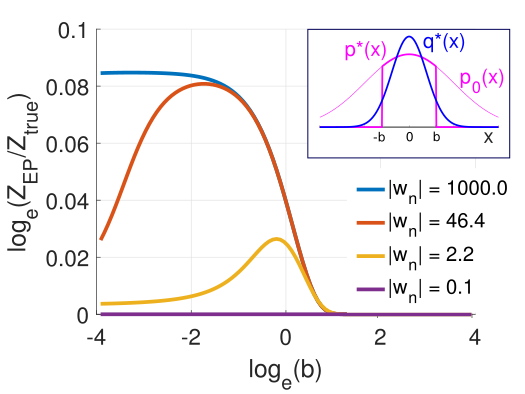
\includegraphics[scale=0.6]{Overestimation_probit_plot.png}
%  \caption{Overestimation of true normalising constant, with 1D probit functions.}
%  \label{fig:Overestimation probit plot}
%\end{figure}
%
%
\begin{figure}[h]
\centering
\begin{subfigure}{.5\textwidth}
  \centering
  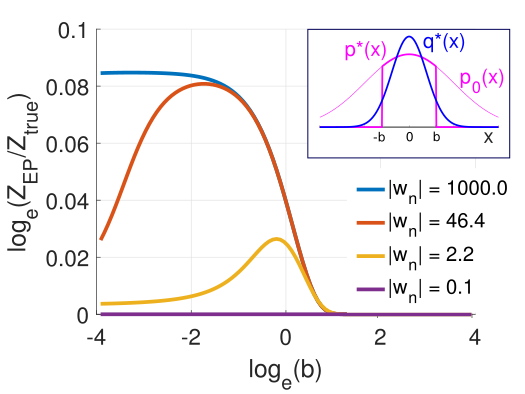
\includegraphics[height=.7\linewidth]{Overestimation_probit_plot.png}
  \caption{Overestimation of true normalising constant,\\ with 1D probit functions (symmetric box case). \\ $p^*(x)$ and $q^*(x)$ are unnormalised $p(x)$ and $q(x)$.}
  \label{fig:Overestimation probit plot}
\end{subfigure}%
\begin{subfigure}{.5\textwidth}
  \centering
  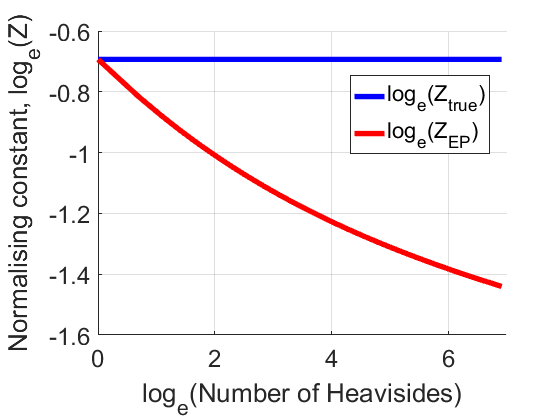
\includegraphics[height=.7\linewidth]{Underestimation_plot.png}
  \caption{Underestimation of true normalising constant\\ as $N$ increases (repeated Heaviside functions).}
  \label{fig:Underestimation probit plot}
\end{subfigure}
\caption{Comparing EP's overestimation and underestimation of the true model evidence.}
\label{fig:Model evidence plots}
\end{figure}
%
\section{Repeated Heaviside functions}
%
The second toy case applies EP to a Gaussian prior multiplied by repeated Heaviside functions (Equation \ref{eq:EP repeated Heavisides}). This is equivalent to an application of Power EP (PEP) \citep{minka_power_2004}: repeating the function $N$ times does not change $p(x)$ ($N \geq 1$), and minimises the $\alpha$-divergence (instead of the $\KLdivK \KLdivL$ divergence) with $\alpha = \frac{2}{N} - 1$. Increasing $N$ reduces $\alpha$ from $\alpha = 1$ (as in EP) towards $\alpha=-1$ (the Variational Inference case). As expected from properties of PEP \citep{minka_divergence_2005}, this approximation increasingly underestimates the normalising constant as $N$ increases, seen in Figure \ref{fig:Underestimation probit plot}. We note that this underestimation is greater than the 10\% overestimation observed in Figure \ref{fig:Overestimation probit plot}, although the underestimation magnitude is decreased slightly when probit functions are used (instead of Heaviside functions), and also when slight jitter (noise) is introduced in the cut-off value between functions (we have only considered $b=0$ for all functions so far).
%
\begin{equation} \label{eq:EP repeated Heavisides}
p(x) = \frac{1}{Z_\mathrm{true}} \left( p_0(x) \prod_{n=1}^N h(- x + 0) \right) \approx \frac{1}{Z_\mathrm{EP}} \left( p_0(x) \prod_{n=1}^N \tilde{t}_{n}(x) \right) = q(x).
\end{equation}
%
Combining the two toy cases considered in a simple 1-dimensional binary classification example illustrates why $Z_\mathrm{EP} \leq Z_\mathrm{true}$ is often observed on realistic datasets. Real world data will tend to be fairly well separated and the likelihood functions in such cases will all have a similar form, meaning the repeated functions case is more prevalent than the symmetric box case. This would cause the repeated functions case's underestimation to overpower any overestimation that may otherwise be observed. It is interesting to note that the two effects can cancel each other out slightly, leading to a value of $Z_\mathrm{EP}$ that is close to $Z_\mathrm{true}$. In \citet{swaroop_understanding_2017} we show that this underestimation does indeed exist for small datasets, and the conjecture is that this expands to larger datasets.
%
\section{FITC}
%
The ‘Fully Independent Training Condition’ (FITC) algorithm is a sparse approximation for Gaussian Process (GP) regression \citep{csato_sparse_2002}, and it has been shown that the solution FITC reaches is the same as that of EP \citep{bui_unifying_2017}. This is a nice application of EP as all factors are Gaussian in FITC, making it amenable to analysis. In fact, it is one of the only cases that the authors know where EP is approximate (it does not return exact inference) but still converges (in a single pass) to an analytic fixed point given by FITC.

The toy case considered here is another counter-example to $Z_\mathrm{EP} \leq Z_\mathrm{true}$. FITC approximates GP regression by using a set of $M$ inducing points to approximate the true dataset, obtained by maximising the FITC likelihood (EP energy) with respect to the inducing points’ locations. It can be shown that $p_\mathrm{FITC}(\vec{y}|\vec{\theta}) = Z_\mathrm{EP}$, and $Z_\mathrm{true} =  p_\mathrm{true}(\vec{y}|\vec{\theta})$ \citep{bui_unifying_2017}.

We consider the case with two training (1-dimensional) input and output pairs, $(x_1, y_1) = (1,0)$ and $(x_2,y_2) = (0,0)$, approximated by $M=2$ inducing points, $(x_{u,1},u_1)$ and $(x_{u_2},u_2)$, with a squared exponential covariance matrix. Figure \ref{fig:FITC} plots the difference in FITC and true likelihoods as we change the input values of the inducing points. The FITC solution is at the maximum of this plot, and we can see that this is not at the true training input locations (marked in red). Having $(x_{u,1},x_{u,2}) = (0.5,0.5)$ is a maximum, as is having one of the inducing input locations ignored (the inducing input has large magnitude) with the other at $0.5$. These FITC solutions therefore satisfy $p_\mathrm{FITC}(\vec{y}|\vec{\theta}) = Z_\mathrm{EP} > Z_\mathrm{true} =  p_\mathrm{true}(\vec{y}|\vec{\theta})$.
%
\begin{figure}[h]
  \centering
  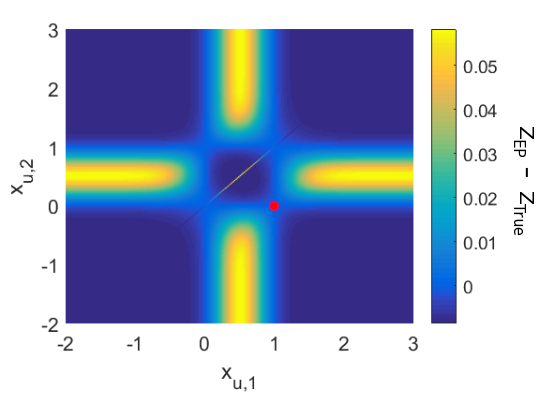
\includegraphics[scale=0.4]{FITC_simple.png}
  \caption{Difference in FITC and true likelihoods (for details, see main text).}
  \label{fig:FITC}
\end{figure}
%

This inexact approximation has been observed before on larger datasets \citep{bauer_understanding_2016, bui_unifying_2017}, and we can use this example to attempt to mathematically characterise it. We compare the behaviour of the terms in the likelihood function, noting their contributions as $\vec{x}$ and $\vec{y}$ change. We find that a determinant term, of the form $\frac{1}{2}\log{|\matr{\Sigma}|}$, prefers an overestimation of the normalising constant, while a quadratic term in $\vec{y}$, of the form $\frac{1}{2}\vec{y}^T\left(\matr{\Sigma}\right)^{-1}\vec{y}$, prefers an overestimation if $y_1=y_2$, and an underestimation if $y_1=-y_2$ \citep{swaroop_understanding_2017}. If the overestimation terms overpower other terms, such as in our example ($\vec{y}=0$), then FITC prefers to ignore an inducing input. Future work could involve considering more training data in order to see how this effect scales mathematically onto larger datasets.
%
\section{Time series} \label{sec:Time Series}
%
The final example applies EP and VI on a simple time series setup, comparing their behaviour. We consider two time-steps of a model comprising two-dimensional latent variables at each time-step (four latent variables in total). The priors are Gaussian $p(x_{d1}) = \mathrm{N}\left(x_{d1};0,\frac{\sigma_x^2}{1-\lambda^2}\right)$, the time-step correlation is $p(x_{d2}|x_{d1}) = \mathrm{N}(x_{d2};\lambda x_{d1},\sigma_x^2)$, and at every time-step we observe $y_t$, $p(y_t|x_{d1},x_{d2}) = \mathrm{N}(y_t;w_1x_{1t} + w_2x_{2t},\sigma_y^2)$. The approximating factors are also Gaussian, ensuring the entire problem is tractable: we can directly compare the approximate inference algorithms with ground truth.

Figure \ref{fig:Time series} plots the correlation between $x_{11}$ and $x_{21}$ as we increase the observation noise $\sigma_y^2$, in the exact case, the EP mean field (MF) approximation (all four variables assumed uncorrelated), the VI MF approximation, and the structured VI approximation (factored across chains, unfactored across time). We have kept the observation weights $w_1$ and $w_2$ at unity for this plot, with $\lambda=0.8$. We see that when $\sigma_y^2$ is very small, there is a high \mbox{(anti-)correlation} between the two variables. Here, the VI approximations are very certain of their predictions (their uncertainty is at the conditional variance of the variables), and EP is much more uncertain (but note that it does not return the marginal uncertainty of the true posterior as some authors suggest). This is a well-known undesired feature of the VI approximation \citep{turner_two_2011}. As the observation noise increases, we see that all the approximations get more uncertain, with EP always being the most uncertain. At high $\sigma_y^2$, the exact distribution tends to the prior, as do the EP and structured VI approximations. The VI MF approximation, however, gets more certain than the prior after observing essentially meaningless data; this seems like a catastrophic failure on its part. For intermediate values of $\sigma_y^2$, both the EP and structured VI approximations seem to provide good approximations to the correlated exact distribution: their uncertainty is between being too certain (the VI MF approximation) and too uncertain (the prior). The nature of the downstream task will determine which of the two approximations is better. However, unlike the structured VI approximation, the EP mean field factorisation is coarser, which can yield computational advantages. See Appendix \ref{app:Time Series} for a comparison of EP and VI when optimising hyperparameters. We find that EP's estimate of model evidence is slightly better than VI's estimate, and EP overestimates the optimal $\lambda^*$.
%
\begin{figure}[h]
  \centering
  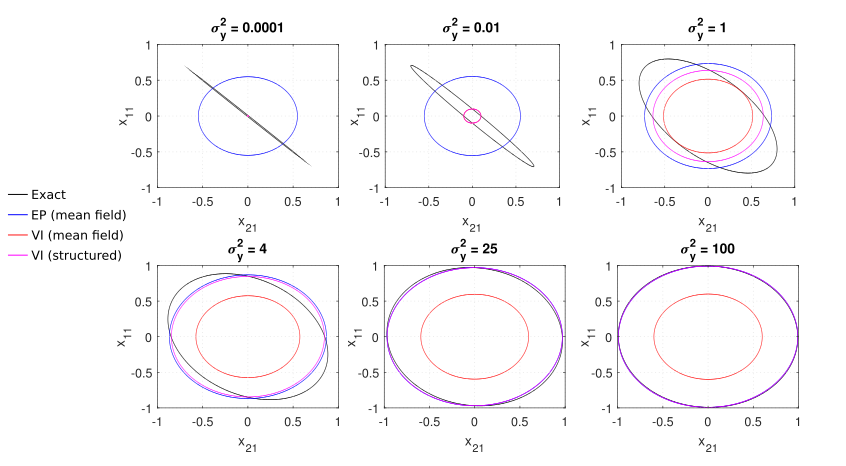
\includegraphics[scale=0.55]{Precision_plots_wrt_sy.png}
  \caption{One standard deviation plots as $\sigma_y^2$ increases.}
  \label{fig:Time series}
\end{figure}
%
\section{Conclusions}
%
We initially looked in detail at the conjecture that $Z_\mathrm{EP}<Z_\mathrm{true}$, presenting the symmetric box case counter-example and arguing why this conjecture may be found on real classification datasets by also considering the repeated Heaviside functions case. The symmetric box case is the first analytic counter-example in the literature. We used the relationship between FITC and EP to find another counter-example to the conjecture, and also used this example to mathematically explain why FITC can prefer to ignore an inducing input. This provides an interesting insight into the FITC algorithm, as one would hope for FITC's inducing inputs to perfectly match the true inputs. In the final toy case, we compared EP and VI's approximations in a simple time series example, finding that the EP mean field approximation retains sensible uncertainty estimates in regimes where mean field VI fails catastrophically. We hope that this work will inspire further work applying approximate inference algorithms to small datasets in order to characterise and analyse them.
%
%\subsubsection*{Acknowledgements}
%
%Use unnumbered third level headings for the acknowledgments. All
%acknowledgments go at the end of the paper. Do not include
%acknowledgments in the anonymized submission, only in the final paper.

\small

\bibliographystyle{abbrvnat}
\bibliography{references}
%
\newpage
%
\titleformat{\section}{\large\bfseries}{\appendixname~\thesection}{0.5em}{}
\appendix
\section{} \label{app:Time Series}
%
This section compares EP mean field (MF) and VI MF approximations when used to optimise a hyperparameter of the time series model introduced in Section \ref{sec:Time Series}. Specifically, we consider optimising the value of $\lambda$ when given the correct values of the other hyperparameters, $\{\sigma_x^2,\sigma_y^2,w_1,w_2\}$. To do this, we set a value for $\lambda_\mathrm{true}$, and calculate the model evidence for EP MF and VI MF. We set $w_1=w_2=1$, $\sigma_y^2=0.43$, $\sigma_x^2=1-\lambda_\mathrm{true}^2$, and use $\lambda_\mathrm{true}$ to calculate the sufficient statistics of $y_1$ and $y_2$.

Figure \ref{fig:Time series hyperparam} shows EP MF, VI MF and exact model evidences as we sweep over different values of $\lambda$. The optimal $\lambda^*$ is given by the maxima of the plots, and is marked with red crosses. As expected, the VI MF model evidence is always less than the true model evidence (VI provides a lower bound), and we also note that VI MF always underestimates $\lambda_\mathrm{true}$ \citep{turner_two_2011}. The EP MF model evidence, however, is much closer to the exact model evidence at all values of $\lambda_\mathrm{true}$ and $\lambda$, while appearing to overestimate the exact model evidence, providing another (empirical) counter-example to the conjecture discussed in the paper. Additionally, the EP MF approximation for $\lambda_\mathrm{true}$ always seems to be an overestimate ($\lambda_\mathrm{EP}^{*} > \lambda_\mathrm{true}$), while also being closer to $\lambda_\mathrm{true}$ than the VI MF.
%
\begin{figure}[h]
  \centering
  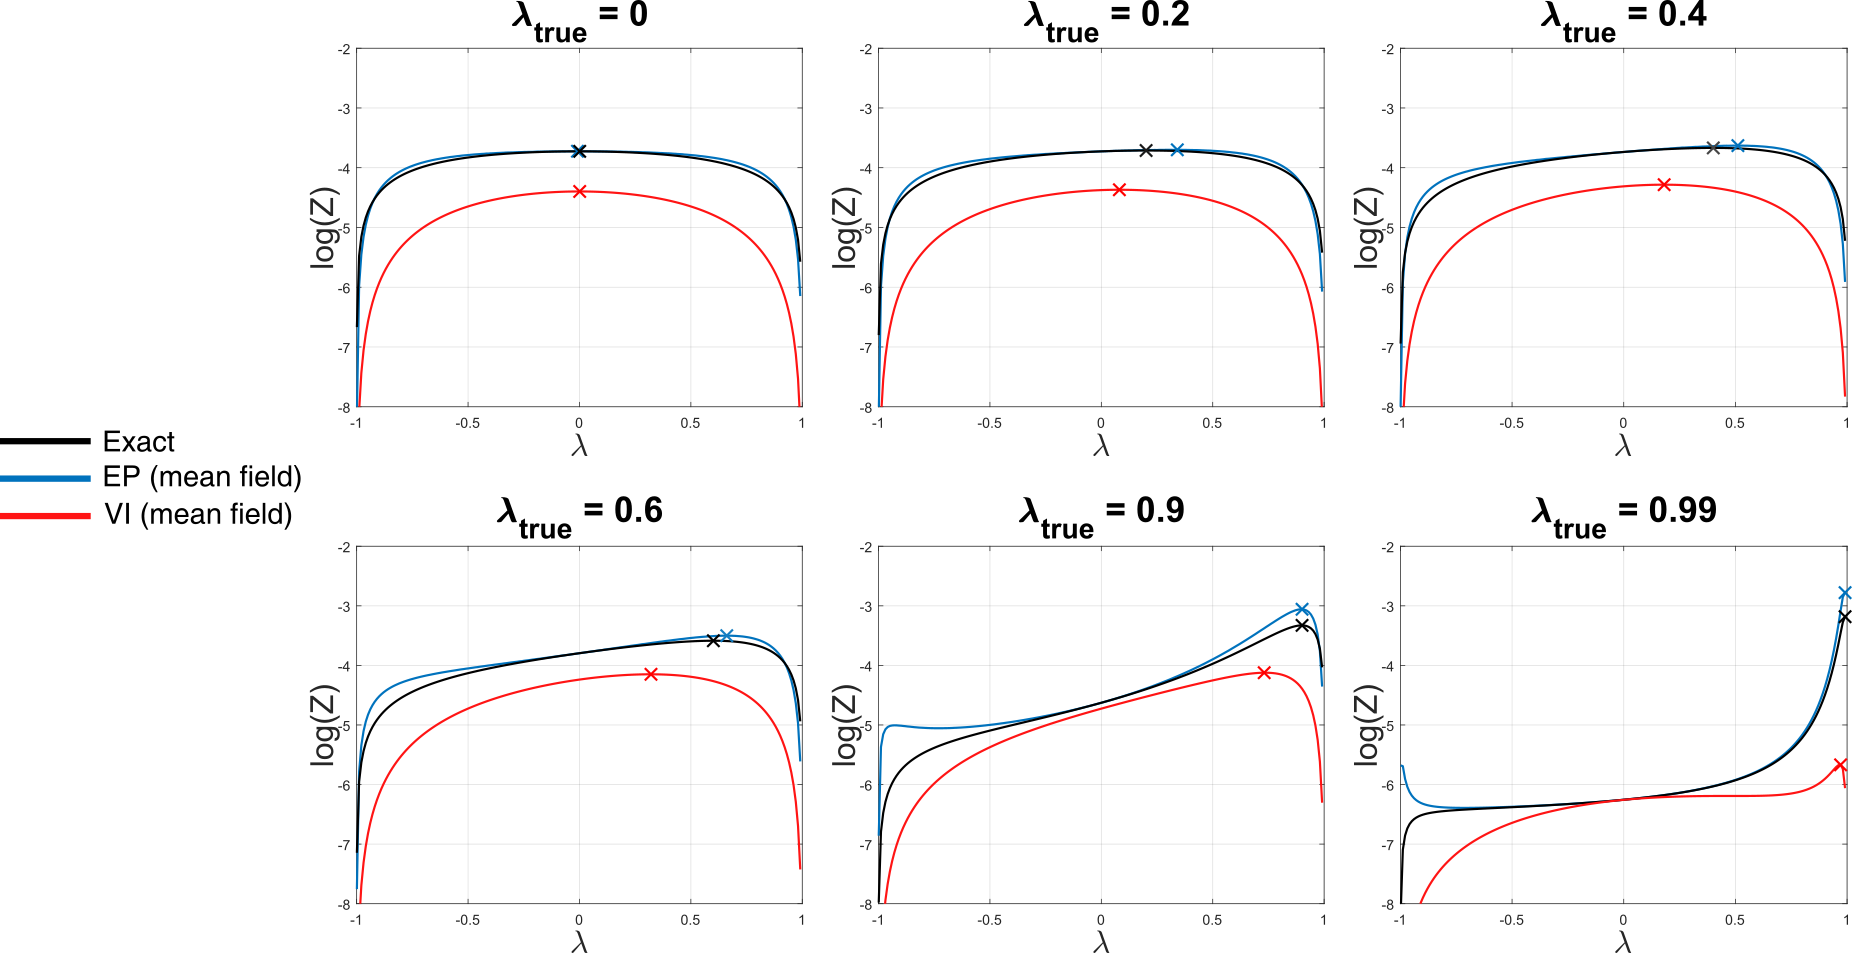
\includegraphics[scale=0.27]{Hyperparam_plots_wrt_lambda.png}
  \caption{EP and VI model evidence plots for optimising $\lambda$.}
  \label{fig:Time series hyperparam}
\end{figure}
%

These preliminary results indicate that the EP MF approximation would be better than VI MF when optimising hyperparameters. Future work would include comparing the EP MF approximations with the structured VI approximation, as in Section \ref{sec:Time Series}. We could also see if the EP MF approximation overestimates the model evidence and the optimal hyperparameter value for other hyperparameters in the model, and when we attempt to optimise more than one hyperparameter at a time. If an overestimation is observed, we could try applying mean field Power EP (with different values of $\alpha$ in the $\alpha$-Divergence) instead of EP or VI to see if we obtain more accurate optimal hyperparameter values. We could also isolate the time correlation $\lambda$ from the variance of the prior, a technique often used in practice, and repeat our tests. Specifically, the equation for the prior changes to $p(x_{d1}) = \mathrm{N}\left(x_{d1};0,\sigma_1^2\right)$, while the time-step correlation $p(x_{d2}|x_{d1})$ and observation $p(y_t|x_{d1},x_{d2})$ are unchanged. It is not clear whether the results in this section will hold with the new time series model, or whether the results are specific to a particular parameterisation.
%
\end{document}